\documentclass{beamer}

\mode<presentation>
{
  \usetheme{Berkeley}
  % or ...

  \setbeamercovered{transparent}
  % or whatever (possibly just delete it)
}

\usepackage{tikz}
\usepackage{graphicx}
\usepackage{wrapfig}
\usepackage[english]{babel}
% or whatever

\usepackage[utf8]{inputenc}
% or whatever

\usepackage{times}
\usepackage[T1]{fontenc}
% Or whatever. Note that the encoding and the font should match. If T1
% does not look nice, try deleting the line with the fontenc.


\title[Implementation: Registration and Version Control with OSF \& GitHub] % (optional, use only with long paper titles)
{Registration and Version Control with OSF \& GitHub}

\subtitle
{Making research more transparent and reproducible}

\author[Garret Christensen] % (optional, use only with lots of authors)
{Garret Christensen\inst{1}}
% - Give the names in the same order as the appear in the paper.
% - Use the \inst{?} command only if the authors have different
%   affiliation.

\institute[Universities of Somewhere and Elsewhere] % (optional, but mostly needed)
{
  \inst{1}%
  Berkeley Initiative for Transparency in the Social Sciences\\
  University of California Berkeley\\
  and\\
  Center for Open Science
}
% - Use the \inst command only if there are several affiliations.
% - Keep it simple, no one is interested in your street address.

\date % (optional, should be abbreviation of conference name)
{BITSS Summer Institute, 2015}
% - Either use conference name or its abbreviation.
% - Not really informative to the audience, more for people (including
%   yourself) who are reading the slides online

\subject{Research Transparency}
% This is only inserted into the PDF information catalog. Can be left
% out. 

% Delete this, if you do not want the table of contents to pop up at
% the beginning of each subsection:
%\AtBeginSubsection[]
%{
%  \begin{frame}<beamer>{Outline}
%    \tableofcontents[currentsection,currentsubsection]
%  \end{frame}
%}

% If you wish to uncover everything in a step-wise fashion, uncomment
% the following command: 
% \beamerdefaultoverlayspecification{<+->}

\begin{document}
    
\begin{frame}
  \titlepage
\end{frame}


%\begin{frame}{Outline}
%  \tableofcontents
  % You might wish to add the option [pausesections]
%\end{frame}

%%%%%%%%%%%%%%%%%%%%%%%%%%%%%%%%%%%%%%%%%%%%%%%%%%%%%%%%%%%%%%%%%%%%%%%%%%%%%%%%%%%%%
\section{Outline}

\begin{frame}[label=main]{Outline}
What have we learned?
\begin{itemize}
\item
Publication bias is a problem.
\hyperlink{supplementalpb}{\beamerbutton{Supplemental}}
\item
P-hacking/specification searching is a problem.
\hyperlink{supplementalhack}{\beamerbutton{Supplemental}}
\item
Registration can help with publication bias.
\item
Pre-analysis plans can help with specification searching.
\item
What should we include in our PAP, and where should we post it?
\end{itemize}
\end{frame}
%%%%%%%%%%%%%%%%%%%%%%%%%%%%%%%%%%%%%%%%%%%%%%%%%%%%%%%%%%%%%%%%%%%%%%%%%%%%%%%%%%%%%
\section{Pre-Analysis Plan}
\begin{frame}{Pre-Analysis Plan}
\pause
\begin{itemize}
\item
Often part of a registration
\item
From 3ie: ``A pre-analysis plan is a detailed description of the analysis to be conducted that is written in advance of seeing the data on impacts of the program being evaluated. It may specify hypotheses to be tested, variable construction, equations to be estimated, controls to be used, and other aspects of the analysis. A key function of the pre-analysis plan is to increase transparency in the research. By setting out the details in advance of what will be done and before knowing the results, the plan guards against data mining and specification searching. Researchers are encouraged to develop and upload such a plan with their study registration, but it is not required for registration.''
\end{itemize}
\end{frame}
%%%%%%%%%%%%%%%%%%%%%%%%%%%%%%%%%%%%%%%%%%%%%%%%%%%%%%%%%%%%%%%%%
\begin{frame}{Origin: FDA's Guidance for Industry}
``E9 Statistical Principles for Clinical Trials'' (1998)
\href{http://www.fda.gov/downloads/drugs/guidancecomplianceregulatoryinformation/guidances/ucm073137.pdf}{\beamergotobutton{Link}}

\S V Data Analysis Considerations
\begin{enumerate}
\item Prespecification of the Analysis
\item Analysis Sets
\item Missing Values and Outliers
\item Data Transformation
\item Estimation, Confidence Intervals, and Hypothesis Testing
\item Adjustment of Significance and Confidence Levels
\item Subgroups, Interactions, and Covariates
\item Integrity of Data and Computer Software Validity
\end{enumerate}
\end{frame}
%%%%%%%%%%%%%%%%%%%%%%%%%%%%%%%%%%%%%%%%%%%%%%%%%%%%%%%%%%%%%%%%
\begin{frame}{Glennerster, Takavarasha Suggestions}
\textit{Running Randomized Evaluations}
\begin{enumerate}
\def\labelenumi{\arabic{enumi}.}
\item
  the main outcome measures,
\item
  which outcome measures are primary and which are secondary,
\item
  the precise composition of any families that will be used for mean
  effects analysis,
\item
  the subgroups that will be analyzed,
\item
  the direction of expected impact if we want to use a one-sided test,
  and
\item
  the primary specification to be used for the analysis.
\end{enumerate}
\end{frame}
%%%%%%%%%%%%%%%%%%%%%%%%%%%%%%%%%%%%%%%%%%%%%%%%%%%%%%%%%%%%%%%%%%%%%%
\begin{frame}{McKenzie Suggestions}
\href{http://blogs.worldbank.org/impactevaluations/a-pre-analysis-plan-checklist}{World Bank Development Impact Blog}

\begin{enumerate}
\item
  Description of the sample to be used in the study
\item
  Key data sources
\item
  Hypotheses to be tested throughout the causal chain
\item
  Specify how variables will be constructed
\item
  Specify the treatment effect equation to be estimated
\item
  What is the plan for how to deal with multiple outcomes and multiple
  hypothesis testing?
\item
  Procedures to be used for addressing survey attrition
\item
  How will the study deal with outcomes with limited variation?
\item
  If you are going to be testing a model, include the model
\item
  Remember to archive it
\end{enumerate}
\end{frame}
%%%%%%%%%%%%%%%%%%%%%%%%%%%%%%%%%%%%%%%%%%%%%%%%%%%%%%%%%%%%%%%
\begin{frame}{Simmons, Nelson, Simonsohn (2011)}
Reporting standards, but related.
\pause
\begin{enumerate}
\item
  Authors must decide the rule for terminating data collection before
  data collection begins and report this rule in the article.
\item
  Authors must collect at least 20 observations per cell or else provide
  a compelling cost-of-data-collection justification.
\item
  Authors must list all variables collected in a study.
\item
  Authors must report all experimental conditions, including failed
  manipulations.
\item
  If observations are eliminated, authors must also report what the
  statistical results are if those observations are included.
\item
  If an analysis includes a covariate, authors must report the
  statistical results of the analysis without the covariate.
\end{enumerate}
\end{frame}
%%%%%%%%%%%%%%%%%%%%%%%%%%%%%%%%%%%%%%%%%%%%%%%%%%%%%%
\begin{frame}{Examples}
Wide range of when to write and how detailed to make the plan. At the extreme level of detail you would have your entire code already written before you got any data.
\begin{itemize}
\item
J-PAL Hypothesis Registry (11), see \url{http://www.povertyactionlab.org/Hypothesis-Registry}
\item
AEA Registry has relatively few, plentiful in EGAP.
\item
Casey, Glennerster, Miguel, ``\href{http://www.nber.org/data-appendix/w17012/GBF_Supplementary_Appendix_2011-10-07.pdf}{Reshaping Institutions: Evidence on Aid Impacts Using a Pre-Analysis Plan}'' \textit{QJE} 2012. (\href{http://http://eml.berkeley.edu/~emiguel/pdfs/miguel_gbf.pdf}{Paper},\href{http://www.nber.org/data-appendix/w17012/GBF_Supplementary_Appendix_2011-10-07.pdf}{Plan})
\begin{itemize}
 \item Government-sponsored program.
 \item Broad program (Community Driven Development)
 \item Broad outcomes (trust, public goods, public services, community groups, information, participation, crime, welfare, attitudes)
 \end{itemize} 
\end{itemize} 
\end{frame}

{ % all template changes are local to this group.
    \setbeamertemplate{navigation symbols}{}
    \begin{frame}[plain]
         \begin{tikzpicture}[remember picture,overlay]
            \node[at=(current page.center)] {
                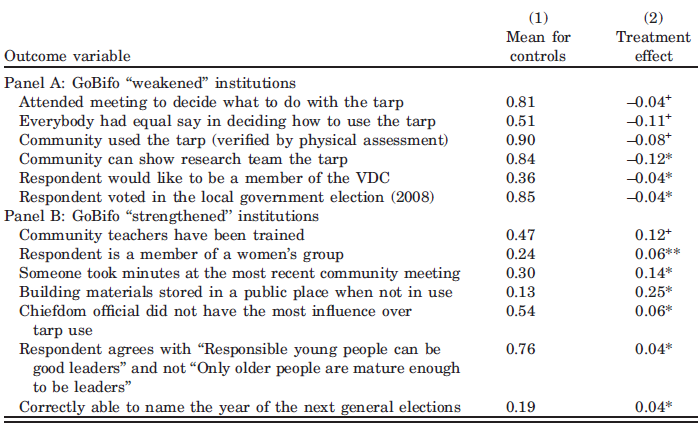
\includegraphics[width=\paperwidth]{GoBifo1.PNG}
            };
        \end{tikzpicture}
     \end{frame}
}
%%%%%%%%%%%%%%%%%%%%%%%%%%%%%%%%%%%%%%%%%%%%%%%%%%%%
\begin{frame}{Why?}
	\begin{itemize}
	\item It's good science; you can distinguish between confirmatory and exploratory analysis.
	\item You get a badge.
	\begin{itemize}
	\item Project Page. \href{https://osf.io/tvyxz/wiki/home/}{\beamerbutton{Link}}
	\item Fertile women aren't more racist (\href{http://pss.sagepub.com/content/26/2/249}{Hawkins, Fitzgerald, Nosek 2015}).
	\end{itemize}
	\item You get \$1000. \href{http://centerforopenscience.org/prereg/}{\beamerbutton{Link}}
	\end{itemize}
\end{frame}
%%%%%%%%%%%%%%%%%%%%%%%%%%%%%%%%%%%%%%%%%%%%%%%%%%%%%%%%%%%%%%%%%%%%%%%%%%%%%%%%%%%%%
\section*{Registrations}
\begin{frame}{Registrations-Medicine}
 \begin{itemize}
  \item
   Publicly stating all research you will do, and what hypotheses you will test, prospectively.
   %\item If we know every hypothesis test that is run on a given subject, we have a better idea of how seriously to take the significant results.
  \item Store this statement in a public registry.
  \item
   Near universal adoption in medical RCTs. Top journals (\href{http://www.nejm.org/doi/full/10.1056/NEJMe048225}{ICMJE}) won't publish if it's not registered.
   \item Largest: \url{http://clinicaltrials.gov}
  \item
   Even better if registry requires registering outcomes after study. Currently limited, and poor compliance (\href{http://www.nejm.org/doi/full/10.1056/NEJMsa1409364}{Anderson et al. 2015}) but NIH is moving on this. \href{http://www.nih.gov/news/health/nov2014/od-19.htm}{\beamerbutton{Link}}
\end{itemize}
\end{frame}

%%%%%%%%%%%%%%%%%%%%%%%%%%%%%%%%%%%%%%%%%%%%%%%%%%%%%%%%%%%%%%%%%%%%%%%%
\begin{frame}[label=regmain]{Registrations-Social Sciences}
\begin{itemize}
   \item Newer to social sciences, but good locations for several fields.
   \item AEA registry, currently only for RCTs. \url{http://socialscienceregistry.org}
   \item
   ``J-PAL supports the American Economic Association's (AEA) registry for randomized controlled trials in economics (http://socialscienceregistry.org). It is a free, easy-to-use database that makes access to trial results more transparent, aims to address the growing number of requests for registration by funders and referees, and helps solve the problem of publication bias by providing a single place where all trials are registered in advance of their start. As of May 31, 2015, the AEA Registry had a total of 379 registered controlled trials in 70 different countries. See how the registry continues to grow below.'' \hyperlink{AEAreg}{\beamerbutton{Link}}
 \end{itemize}
 \end{frame}
%%%%%%%%%%%%%%%%%%%%%%%%%%%%%%%%%%%%%%%%%% 
 \begin{frame}{Registrations-Social Sciences}
 \begin{itemize}
   \item
    EGAP registry \url{http://egap.org/design-registration}
   \item 
    3ie registry, for developing country evaluations. \url{http://ridie.3ieimpact.org}
   \item
   	Open Science Framework \url{http://osf.io}
   	\begin{itemize}
   	\item
   	Open format
   	\item
   	Will soon sync with above
   	\item
   	Version Control!
   	\end{itemize}
   \end{itemize}  
\end{frame}
%%%%%%%%%%%%%%%%%%%%%%%%%%%%%%%%%%%%%%%%%%%%%%%%%%%%%%%%%%%%%%%%%%%%%%%%%%%%%%%%%%%%%
{ % all template changes are local to this group.
    \setbeamertemplate{navigation symbols}{}
    \begin{frame}[plain]
        \begin{tikzpicture}[remember picture,overlay]
            \node[at=(current page.center)] {
                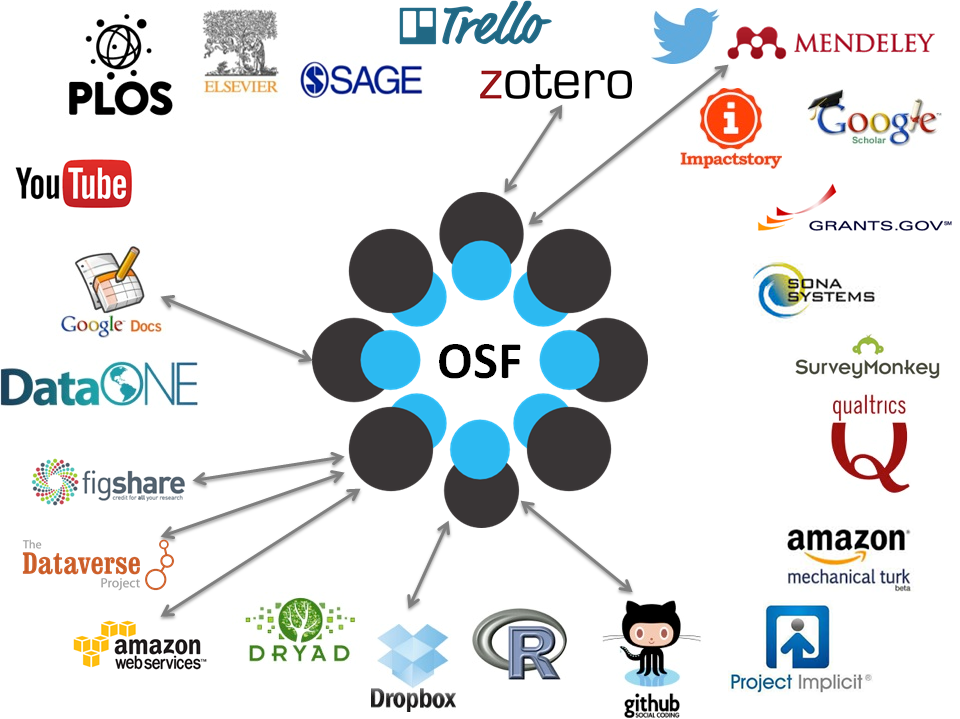
\includegraphics[height=\paperheight]{OSFnow.PNG}
            };
        \end{tikzpicture}
     \end{frame}
 % all template changes are local to this group.
    \setbeamertemplate{navigation symbols}{}
    \begin{frame}[plain]
        \begin{tikzpicture}[remember picture,overlay]
            \node[at=(current page.center)] {
                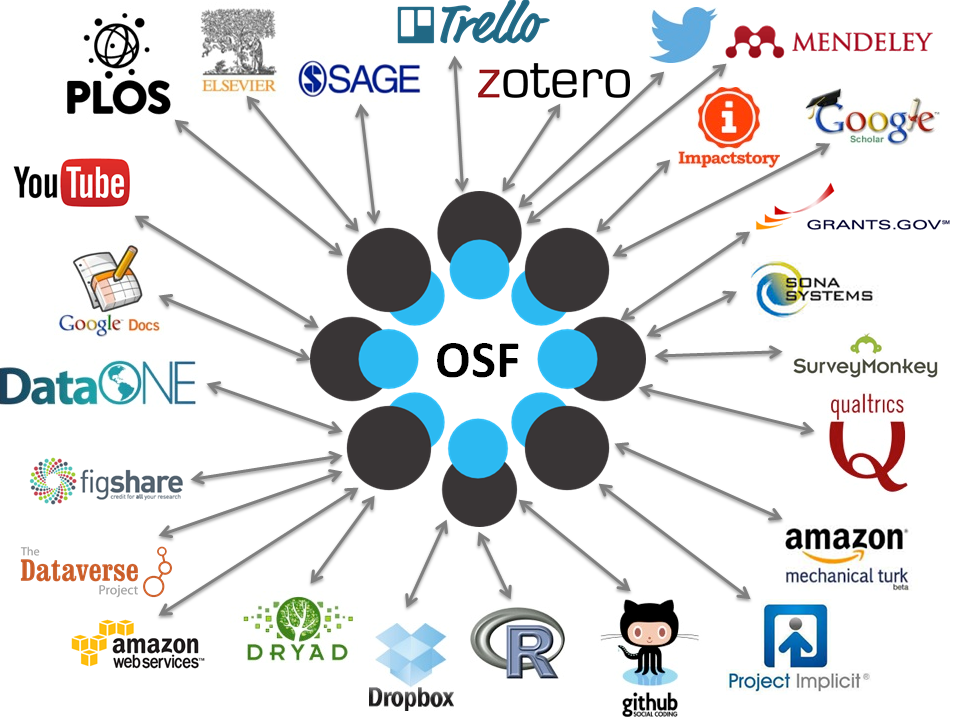
\includegraphics[height=\paperheight]{OSFsoon.PNG}
            };
        \end{tikzpicture}
     \end{frame}
}
%%%%%%%%%%%%%%%%%%%%%%%%%%%%%%%%%%%%%%%%%%%%%%%%%%%%%%%%%%%%%%%%%%%%%%%%
\begin{frame}{OSF Demo}
\begin{itemize}
\item Create a Project.
\item Add a collaborator.
\item Upload a file.
\item Edit and save the file, without changing the name.
\item Upload the file again.
\item Link project to GitHub repo.
\end{itemize}
\end{frame}
%%%%%%%%%%%%%%%%%%%%%%%%%%%%%%%%%%%%%%%%%%%%%%%%%%%%%%%%%%%%%%%%%%%%%%%%%%%%%%%%%%%
\begin{frame}{Version Control}
\begin{wrapfigure}[6]{r}[0pt]{3cm}

\includegraphics[width=0.9\linewidth]{github-logo-transparent.jpg}
\end{wrapfigure}
Why use version control?

  \href{http://stackoverflow.com/questions/1408450/why-should-i-use-version-control}{\beamerbutton{StackOverflow}}
\begin{itemize}
\item Backup
\item Forking
\item Rewinding
\item Collaboration
\item GitHub: extremely powerful--how open source coding happens. Still easy enough for single-person light coding.
\end{itemize}

\end{frame}

%%%%%%%%%%%%%%%%%%%%%%%%%%%%%%%%%%%%%%%%%%%%%%%%%%%%%%%%%%%%%%%%%%%%%%%%%%%%%%%%
\begin{frame}{GitHub Demo}
\begin{wrapfigure}[6]{r}[0pt]{3cm}

\includegraphics[width=0.9\linewidth]{github-logo-transparent.jpg}
\end{wrapfigure}
Use GitHub to:
\begin{itemize}
\item Create a repo.
\item Change a file.
\item Add, Commit, Push.
\item Do group work.
\begin{itemize}
 \item Add a collaborator (they get direct permission).
 \item Pull requests (how open source works).
\end{itemize}
\end{itemize}
\end{frame}
%%%%%%%%%%%%%%%%%%%%%%%%%%%%%%%%%%%%%%%%%%%%%%%%%%%%%%%%%%%%%%%%%%%%%%%%%%%%%%%%%%%%%
\section{Conclusion}
\begin{frame}{Conclusion}
 \begin{itemize}
 \item
  Register your work to reduce publication bias. 
 \item
  Include a pre-analysis plan to reduce researcher degrees of freedom.
 \item
  Register in most appropriate site for your work, OSF will hold anything, and link to your entire workflow.
  \item
  Use version control (GitHub, BitBucket, etc.).
  \item
  Share your data (Harvard Dataverse--Alex Wais next).
\end{itemize}

\end{frame}
%%%%%%%%%%%%%%%%%%%%%%%%%%%%%%%%%%%%%%%%%%%%%%%%%%%%%%%%%%%%%%%%%%%%%%%%%%%%%%
%%%%%%%%%%%%%%%%%%%%%%%%%%%%%%%%%%%%%%%%%%%%%%%%%%%%%%%%%%%%%%%%%%%%%%%%%%%%%%%
\appendix
\section{Supplemental-Publication Bias}
\begin{frame}[label=supplementalpb]{Supplemental: Publication Bias}
  \begin{itemize}
  %\item
   %The distibution of published p-values jumps around .05 (Brodeur et al 2013).
  \item
  There is a higher fraction of rejected hypothesis tests in the social sciences than in physical sciences (Fanelli 2010).
  \item
  	Published null results are disappearing over time, in all disciplines (Fanelli 2011). 
  \item
    This is very unlikely to represent the true state of the universe.
  \item
  	Data on the full set of experiments run with a large survey shows strong results are 40pp more likely to be published, and 60pp more likely to be written up. The file drawer problem is massive. (Franco, Malhotra, Simonovits 2014)
  \end{itemize}
 \end{frame}
  
  \begin{frame}{Supplemental: Publication Bias}
  If we only write up/publish significant results, and we have no record of all the insignificant results, we have no way to tell if our `significant' results are real, or if they're the 5\% we should expect due to randomness.
\vspace{0.25in}

Back to \hyperlink{main}{\beamerbutton{main}}.
\end{frame}
%%%%%%%%%%%%%%%%%%%%%%%%%%%%%%%%%%%%%%%%%%%%%%%%%%%%%%%%%%%%%%%%%%%%%%%%%%%%%%%%%

\section{P-Hacking}
\begin{frame}[label=supplementalhack]{Supplemental: P-Hacking}
\begin{itemize}
\item
Also called fishing, researcher degrees of freedom, data mining, data massaging, data dredging, or specification searching.
\item
Definition: flexibility in data analysis allows portrayal of \textit{anything} as below an arbitrary p-value threshhold; significance loses its meaning.
\item
Not something only evil people do. It can be subconcious---humans are really good at motivated reasoning.
\item
Not just that, we make completely reasonable but data-dependent decisions (Gelman, Loken 2013/2014 ``Garden of Forking Paths'')
\end{itemize}
\end{frame}


\begin{frame}{Supplemental: P-Hacking}
\begin{itemize}
\item
Do people actually do this? (Previous---John, Loewenstein, Prelec 2011)
\item
Listening to the Beatles' ``When I'm Sixty-Four'' makes you younger. (Simmons, Nelson, Simonsohn 2011)
\item
Inordinately many .049 p-values, and indordinately few .051's; 10-20\%. (Brodeur et al 2015, ``Star Wars'')
\item 
Political ideologues literally see in black and white (Nosek, Spies, Motyl 2012)
\end{itemize}

\vspace{0.25in}
Back to \hyperlink{main}{\beamerbutton{main}}.

\end{frame}

%%%%%%%%%%%%%%%%%%%%%%%%%%%%%%%%%%%%%%%%%%%%%%%%%%%%%%%%%%%%%%%%%%%

{ % all template changes are local to this group.
    \setbeamertemplate{navigation symbols}{}
    \begin{frame}[plain, label=AEAreg]
         \begin{tikzpicture}[remember picture,overlay]
            \node[at=(current page.center)] {
                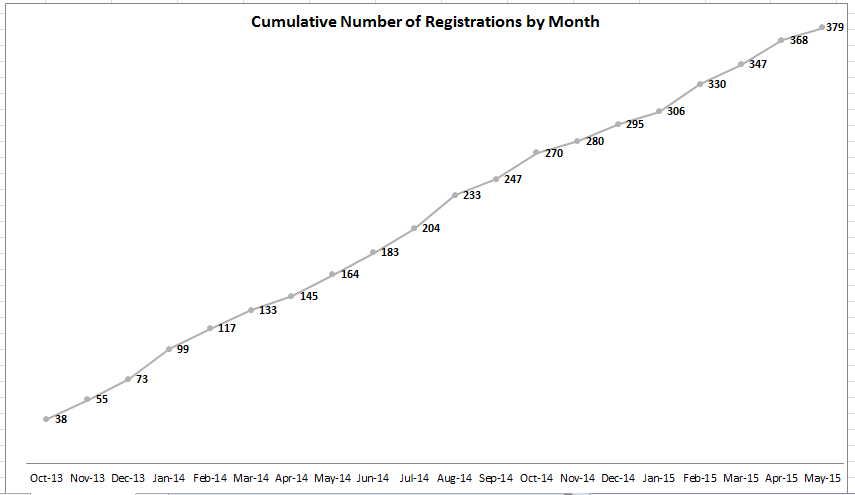
\includegraphics[width=\paperwidth]{AEAreg.png}
            };
        \end{tikzpicture}
        \hyperlink{regmain}{\beamerbutton{main}}
     \end{frame}
}


%%%%%%%%%%%%%%%%%%%%%%%%%%%%%%%%%%%%%%%%%%%%%%%%%%%%%%%%%%%%%%%%%%%%%%%%%%%%%%%%%%%%%%%
\end{document}


